%debseal_HW2 <- function() {
%Sweave("debseal_HW2.Rnw")
%system(paste("pdflatex --interaction=nonstopmode",  "debseal_HW2.tex"))
%shell.exec(file.path(getwd(), "debseal_HW2.pdf"))
%}


\documentclass{article}
\topmargin 0pt
\advance \topmargin by -\headheight
\advance \topmargin by -\headsep
\textheight 8.9in
\usepackage{amsmath}
\usepackage{amsfonts}
\usepackage[noae]{Sweave}
\usepackage{enumerate}
\oddsidemargin 0pt
\evensidemargin \oddsidemargin

\begin{document}
\title{ CSCI-B 565 DATA MINING \\
Homework 2 \\
Morning Class\\
Computer Science Core\\Fall 2013\\Indiana University}
\author{ Debpriya Seal\\ debseal@indiana.edu}
\maketitle
All the work herein is solely mine. \\

R code to get environment ready: \\
\begin{Schunk}
\begin{Sinput}
> defDir <- getwd()
> #newDir <- "debseal"
> #dir.create(file.path(defDir, newDir),showWarnings = FALSE)
> setwd(file.path(defDir))
> if(is.element("HSAUR2", installed.packages()[,1])) { 
+ 	print("HSAUR2 package already installed") 
+ } else {
+ 	print("Installing Package HSAUR2 ....") 
+ 	install.packages('HSAUR2')
+ }
\end{Sinput}
\begin{Soutput}
[1] "HSAUR2 package already installed"
\end{Soutput}
\begin{Sinput}
> if(is.element("alr3", installed.packages()[,1])) { 
+ 	print("alr3 package already installed") 
+ } else {
+ 	print("Installing Package alr3 ....") 
+ 	install.packages('alr3')
+ }
\end{Sinput}
\begin{Soutput}
[1] "alr3 package already installed"
\end{Soutput}
\begin{Sinput}
> if(is.element("tm", installed.packages()[,1])) { 
+ 	print("tm package already installed") 
+ } else {
+ 	print("Installing Package tm ....") 
+ 	install.packages('tm')
+ }
\end{Sinput}
\begin{Soutput}
[1] "tm package already installed"
\end{Soutput}
\begin{Sinput}
> require(lattice)
> library("HSAUR2")
> library("alr3")
> library("tm")
> data(USstates)
> data(banknote)
> print("R Environment set ready") 
\end{Sinput}
\begin{Soutput}
[1] "R Environment set ready"
\end{Soutput}
\end{Schunk}
\section*{Problems}
\begin{enumerate}
	\item[Problem] 1  
		The following problems have to do with metrics. In each case, prove or disprove the distance is a metric.\\
	\emph{Answer:} A \emph{metric} on a set X is a function $d  X \times X \to R$ such that:
	\begin{enumerate}[(i)]
			\item $d(x, y) \ge 0$ for all $x, y \in X$;
			\item $d(x, y) = 0$ if and only if  $x = y$;
			\item $d(x, y) = d(y, x)$ for all $x, y \in X,$ and;
			\item $d(x, y) \ge d(x, z) + d(z, y)$ for all $x, y, z \in X$
	\end{enumerate}
	\begin{enumerate}[(a)]
			\item Lets  see whether the below distance is a metric or not\\
			$d(x, y) = max\{\mid x_i - y_i\mid\}, \forall  1 \le i \le n$ \\
			In order to prove it is metric, we need to make sure that the above 4 properties are met. Let us see them one by one,\\
			\begin{enumerate}[(i)]
			\item $d(x, y) \ge 0$ for all $x, y \in X$: This is true since we are taking the modulus of it. Hence, it can never be less than 0.
			\item $d(x, y) = 0$ if and only if  $x = y$: Clearly since we are doing subtraction operation here. For it to be 0, $x=y$.
			\item $d(x, y) = d(y, x)$ for all $x, y \in X$:  Again the modulus came to rescue. Since, we are taking modulus, it really doesn't matter we take perform $x-y$ or $y-x$.
			\item $d(x, y) \ge d(x, z) + d(z, y)$ for all $x, y, z \in X$: \\
				$d(x, z) = max| x_j - z_j |$ for some j \\		
						$\le max|x_j - y_j| + max|y_j - z_j|$  (Since, $|p + q| \le |p| + |q|$)\\ 
						$\le d(x, y) + d(y, z)$
			\end{enumerate}


			\item \\
			\emph{Answer:} Lets see whether the below distance preserves all the 4 metric rule. \\
			$d(x,y) = \sum^{n}_{i} \frac{c(x_{i}, y_{i})}{i}, \forall 1 \le i \le n$
			\begin{enumerate}[(i)]
			\item $d(x, y) \ge 0$ for all $x, y \in X$: Since c function only yields 0 or 1 and we are performing summation alone. Hence, it can never be less than 0.
			\item $d(x, y) = 0$ if and only if  $x = y$: Again $d(x,y)$ will be 0 only if the summation turns out to 0. For it to be 0, $x=y$.
			\item $d(x, y) = d(y, x)$ for all $x, y \in X$:  Since c function checks for inequality alone.It really doesn't matter we take perform $x\neq y$ or $y\neq x$.
			\item $d(x, y) \ge d(x, z) + d(z, y)$ for all $x, y, z \in X$: \\
				$d(x, z) = \sum^{n}_{i} \frac{c(x_{i}, z_{i})}{i}$ for some j \\		
						 $\le \sum^{n}_{i} \frac{c(x_{i}, y_{i})}{i} + \sum^{n}_{i} \frac{c(y_{i}, z_{i})}{i}$ (Because since we are only adding positive quantity.)
						 $\le d(x_i,y_i) + d(y_i,z_i)$
			\end{enumerate}

			\item \\
			\begin{enumerate}
				\item  $d_0 \times d_1$ \\
				Answer: Lets see whether the below operation on 2 metrics preserves all the 4 metric rule. \\	
			\begin{enumerate}[(i)]
			\item $d(x, y) \ge 0$ for all $x, y \in X$: Since we know $d_0, d_1$ are metrics with R_{$\ge 0$}. Even the cartesian product would be greater than 0.
			\item $d(x, y) = 0$ if and only if  $x = y$: Clearly, when $d_0$ and  $d_1$ are equal only then they would be equal
			\item $d(x, y) = d(y, x)$ for all $x, y \in X$:  Since, we are taking cartesian product.It really doesn't matter we take perform $x\times y$ or $y\times x$.
			\item $d(x, y) \ge d(x, z) + d(z, y)$ for all $x, y, z \in X$: \\
			\end{enumerate}
		
	
				\item  $(d_0 + d_1)/d_{0}d_{1}$ \\
				Answer: Lets see whether the below operation on 2 metrics preserves all the 4 metric rule. \\	
			\begin{enumerate}[(i)]
			\item $d(x, y) \ge 0$ for all $x, y \in X$: Since we are dealing with only positive reals. We are good with this.
			\item $d(x, y) = 0$ if and only if  $x = y$: 
			\item $d(x, y) = d(y, x)$ for all $x, y \in X$:  Since we are doing adding and multiplication.We preserve this.
			\item $d(x, y) \ge d(x, z) + d(z, y)$ for all $x, y, z \in X$: \\
			\end{enumerate}
		
			\end{enumerate}
			
			\item  $max\{d_0,d_1\}$ \\
			Answer: Lets see whether the below operation on 2 metrics preserves all the 4 metric rule. \\	
			\begin{enumerate}[(i)]
			\item $d(x, y) \ge 0$ for all $x, y \in X$: Since both of them are metrics by themselves. This is hold true.
			\item $d(x, y) = 0$ if and only if  $x = y$: This is maintained trivially.
			\item $d(x, y) = d(y, x)$ for all $x, y \in X$:  With max operation it really does'nt matters.
			\item $d(x, y) \ge d(x, z) + d(z, y)$ for all $x, y, z \in X$: \\
			\end{enumerate}			
			
			
			\item  $d(x,y) =  \frac{||x \cap y||}{||x \cup y|| + 1} $ \\
			Answer: Lets see whether the below operation on 2 metrics preserves all the 4 metric rule. \\	
			\begin{enumerate}[(i)]
			\item $d(x, y) \ge 0$ for all $x, y \in X$: Since we are dealing with positive real number.We are good with this.
			\item $d(x, y) = 0$ if and only if  $x = y$:This is not preserved. As for d(x,y) to be zero x and y needs to be different.

			\end{enumerate}			
			\emph{Answer:}
		\end{enumerate}

	\item[Problem] 2 Consider the relation in Fig. 1. Partition this data into three blocks using exactly three attributes (or features). For attributes X, Y , use L2. For A use Jaccard Index. For attribute Z you are free to pick a metric. The table has not been cleaned nor transformed. \\
	\emph{Answer:} Lets compute the Jaccards Index for A. Jaccards Index is given by: \\
	where $A = \{a, b, c, d, e, f\}$. \\
	But we see that we have even g in there.I will assume that g is the noise and completely discard it.
	Computing Jaccards Index:\\
	$
	J(SetX) = \frac{f_11}{f_10 +f_01 + f_11} \\
	1) abcd= {1,1,1,1,0,0} \\
	2) bcde= {0,1,1,1,1,0} \\
	3) bcd= {0,1,1,1,0,0} \\
	4) acde= {1,0,1,1,1,0} \\
	5) bdf= {0,1,0,1,0,1} \\
	6) fg= {0,0,0,0,0,1} (Discarded g) \\
	7) abf= {1,1,0,0,0,1} \\
	
	J(1,2) = 3/5 \\
	. \\
	. \\
	$
	
	Now lets compute Eculidean Distance.\\
	$ x,y \in X \\
	d(x,y) = \sqrt(x-y)^2 \\
	d(x,y) = \sqrt(x_1-y_2)^2 \implies \sqrt(1-3)^2 \\
	d(x,y) = \sqrt(x_1-y_2)^2 \implies \sqrt(3-4)^2 \\
	. \\
	. \\
	. \\
	$
	For Z, i am going with Binary metrics i.e \\
	\[ Z = \left\{ 
  \begin{array}{l l}
    0 & \quad \text{if Z == N}\\
    1 & \quad \text{o.w.}
  \end{array} \right.\]
	
Now we just need to compute the similarity for this.\\
	
	\item[Problem] 3  From Everitt, exercise 2.3,2.4.
		\begin{enumerate}
			\item[2.3] D\\
			\emph{Answer:}
\begin{Schunk}
\begin{Sinput}
> plot(USstates)
\end{Sinput}
\end{Schunk}
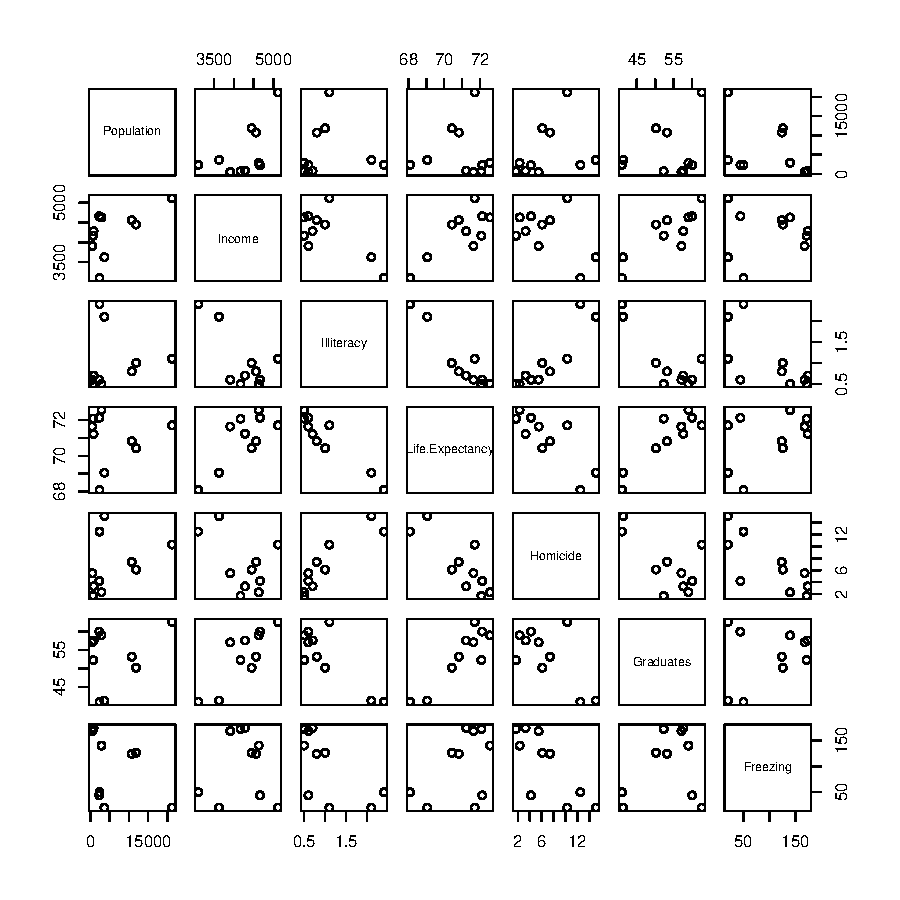
\includegraphics{debseal_HW2-002}
			\item[2.4] E\\
			\emph{Answer:} \\
			\begin{center}
\begin{Schunk}
\begin{Sinput}
> nf <- layout(matrix(c(2,1,2,1), 2, 2, byrow=TRUE), respect=TRUE)
> boxplot(Left ~ Y, data=banknote, xlab= "Counterfeit or not", ylab="Left Margin of note")
> boxplot(Right ~ Y, data=banknote, xlab= "Counterfeit or not", ylab="Right Margin of note")
> boxplot(Diagonal ~ Y, data=banknote, xlab= "Counterfeit or not", ylab="Top Margin of note")
> boxplot(Top ~ Y, data=banknote, xlab= "Counterfeit or not", ylab="Top Margin of note")
> boxplot(Bottom ~ Y, data=banknote, xlab= "Counterfeit or not", ylab="Bottom Margin of note")
\end{Sinput}
\end{Schunk}
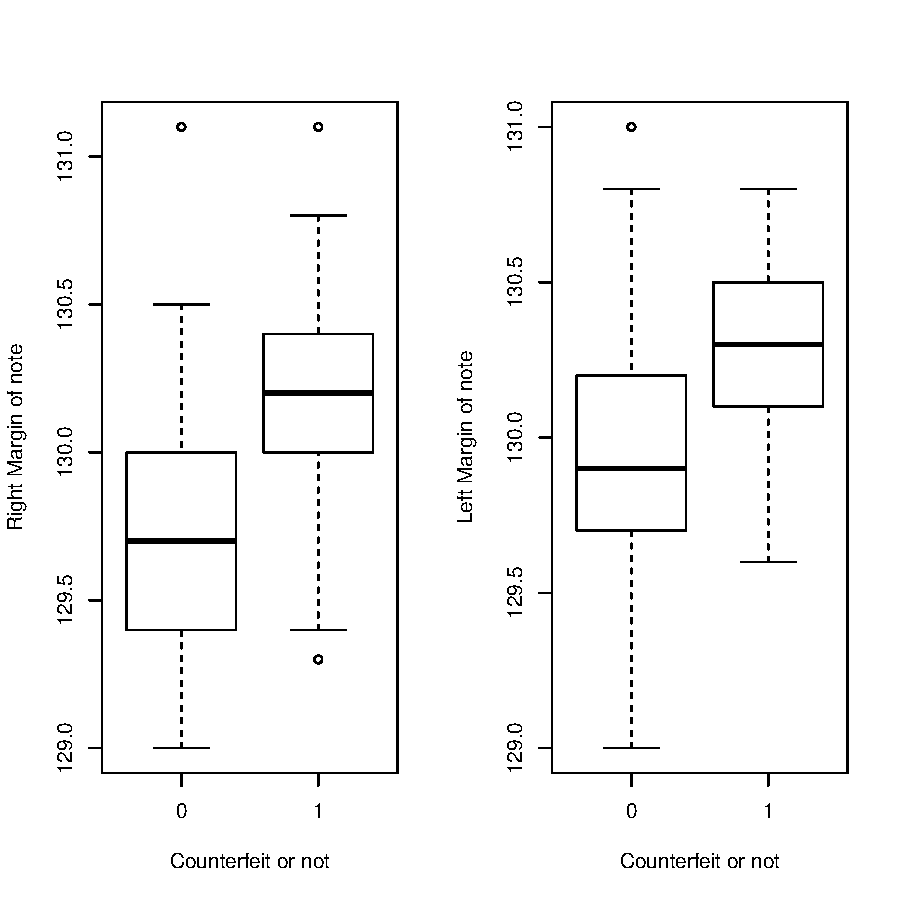
\includegraphics{debseal_HW2-003}

			\end{center}
		\emph{\textfb{My Findings}}: All the margins are way too wide for counterfeit. As you can see the shift in mean.\\
		However, the diagonal length rather small for counterfeit notes compared to original.
		\end{enumerate}		

	\item[Problem] 4 We have provided data from the FHA, "FHA Single Family Loan Performance Trends, Credit Risk Report," June 2013.
		\begin{enumerate}
			\item Put the table Share By Reason for Delinquency in Percent into an R data frame.\\
			\emph{Answer:}
\begin{Schunk}
\begin{Sinput}
> FHA_Table1 <- read.csv("FHA_Table1.csv")
> class(FHA_Table1)
\end{Sinput}
\begin{Soutput}
[1] "data.frame"
\end{Soutput}
\end{Schunk}
			\begin{enumerate}
				\item Plot Reduction of Income against Unemployed. Discuss the results.\\
				\emph{Answer:}
					\begin{center}
\begin{Schunk}
\begin{Sinput}
> plot(FHA_Table1[,3], FHA_Table1[,4], ylab="Unemployed", xlab="Reduction of Income")
\end{Sinput}
\end{Schunk}
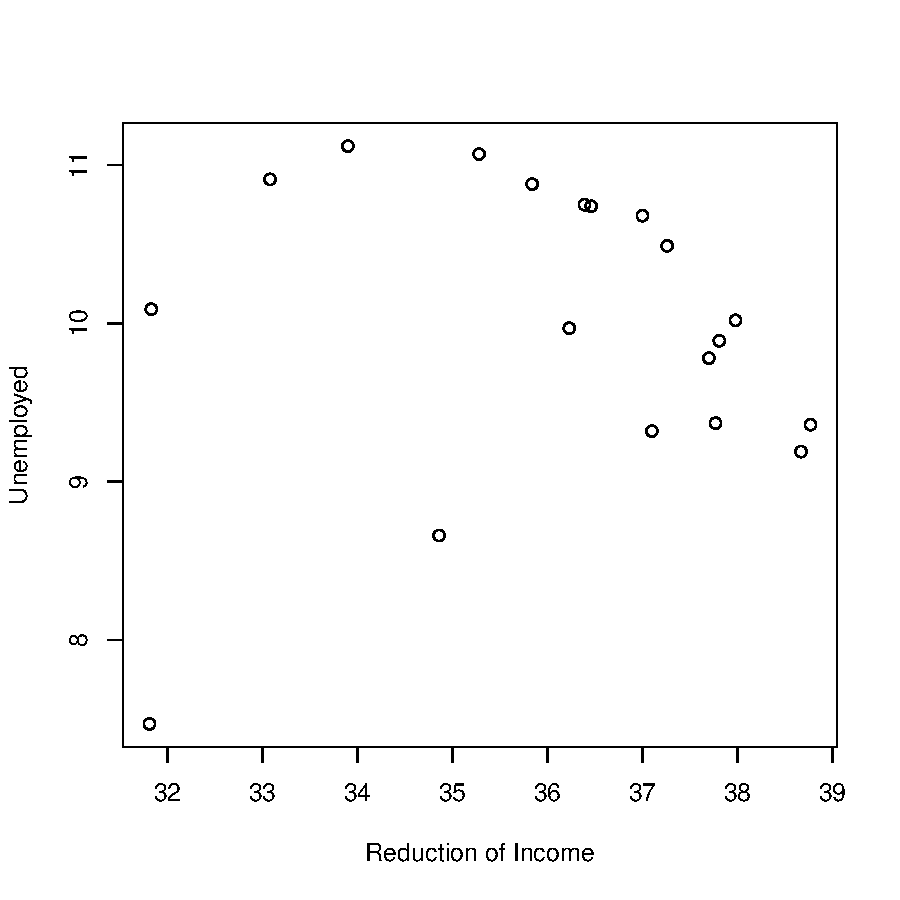
\includegraphics{debseal_HW2-005}
					\end{center}
					\textbf{\emph{Results:}} Here with some noise/outliers we can see that the correlation is negative. In orther words, we can see
					that with increase in Unemploment the Rate of Income is falling.
				\item Plot Death against Unemployed. Discuss the results.\\
				\emph{Answer:} 
					\begin{center}
\begin{Schunk}
\begin{Sinput}
> plot(FHA_Table1[,6], FHA_Table1[,4], ylab="Unemployed", xlab="Death")			
\end{Sinput}
\end{Schunk}
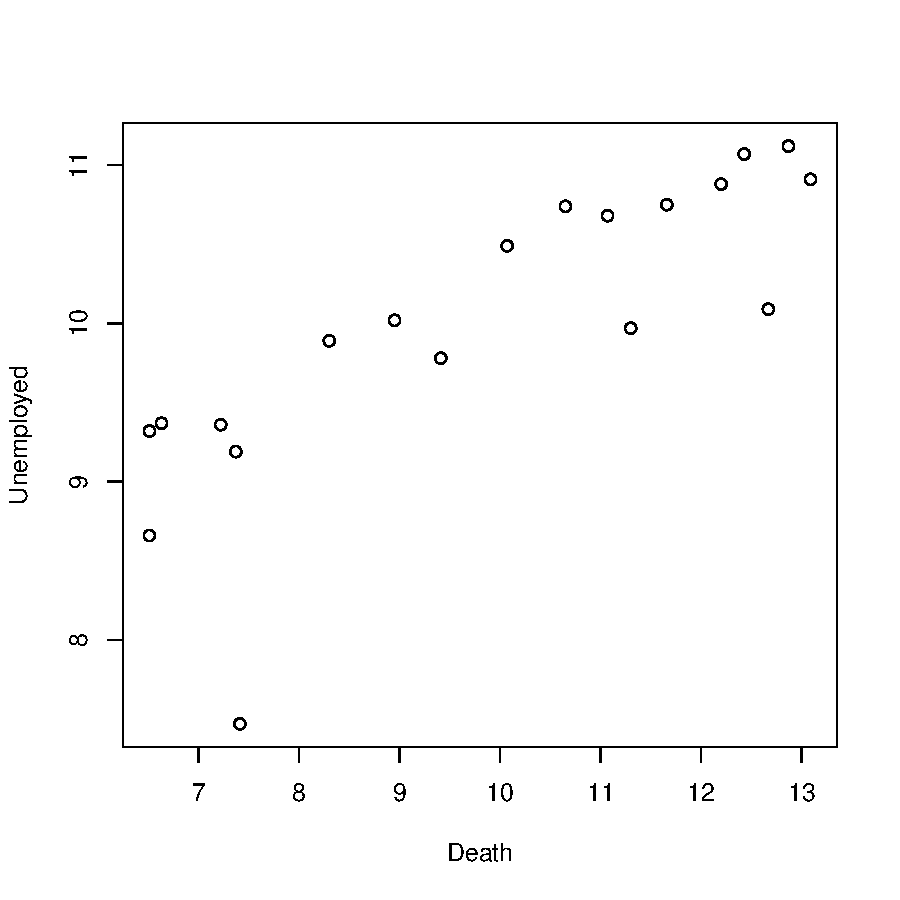
\includegraphics{debseal_HW2-006}
					\end{center}
				\textbf{\emph{Results:}} Clearly, we can see  positive correlation between the increase in Unemployment and increase in death rate.And it makes complete sense as well. Unemployment has been attributed as one of the reason for increase in death rate.
			\end{enumerate}				
			
			\item Put the subtable Credit Score Range in the Delinquency Rates into an R data frame.\\
			\emph{Answer:}
\begin{Schunk}
\begin{Sinput}
> FHA_Table2 <- read.table("FHA_Table2.csv",sep=",", colClasses=c("character", "numeric","numeric","numeric","numeric","numeric","numeric","numeric","numeric"), header=TRUE)	
> class(FHA_Table1)
\end{Sinput}
\begin{Soutput}
[1] "data.frame"
\end{Soutput}
\end{Schunk}
			\begin{enumerate}
				\item Using R find the number of loans with credit scores less than 620.\\
				\emph{Answer:}
					\begin{center}
\begin{Schunk}
\begin{Sinput}
> FHA_Table2$Credit <- sapply(FHA_Table2$Credit, as.character)
> indexDash <- regexpr("-",FHA_Table2$Credit)
> creditHighEnd <- substr(FHA_Table2$Credit, indexDash+1, nchar(FHA_Table2$Credit))
> creditHighEnd <- as.numeric(gsub("\\D", "", creditHighEnd))
> FHA_Table2$creditHighEnd <- creditHighEnd
> creditBelow620 <- subset(FHA_Table2[-1,],creditHighEnd < 620 )
> FHA_Table2[1,2] * sum(creditBelow620$IIF_Shares) / 100
\end{Sinput}
\begin{Soutput}
[1] 659604.8
\end{Soutput}
\end{Schunk}
					\end{center}

				\item Of these loans, how many are past due?\\
				\emph{Answer:}
					\begin{center}
\begin{Schunk}
\begin{Sinput}
> creditBelow620$IIF_Shares_Value <- FHA_Table2[1,2] * creditBelow620$IIF_Shares
> sum(creditBelow620$IIF_Shares_Value * creditBelow620$All_Past_Dues/100)
\end{Sinput}
\begin{Soutput}
[1] 25923717
\end{Soutput}
\end{Schunk}
					\end{center}

				\item Plot Credit Score against All Past Due.\\
				\emph{Answer:}
					\begin{center}
\begin{Schunk}
\begin{Sinput}
> bins <- sapply(FHA_Table2[-1,1], as.factor)
> bins <- ordered(bins)
> plot(bins, FHA_Table2[-1,3])
\end{Sinput}
\end{Schunk}
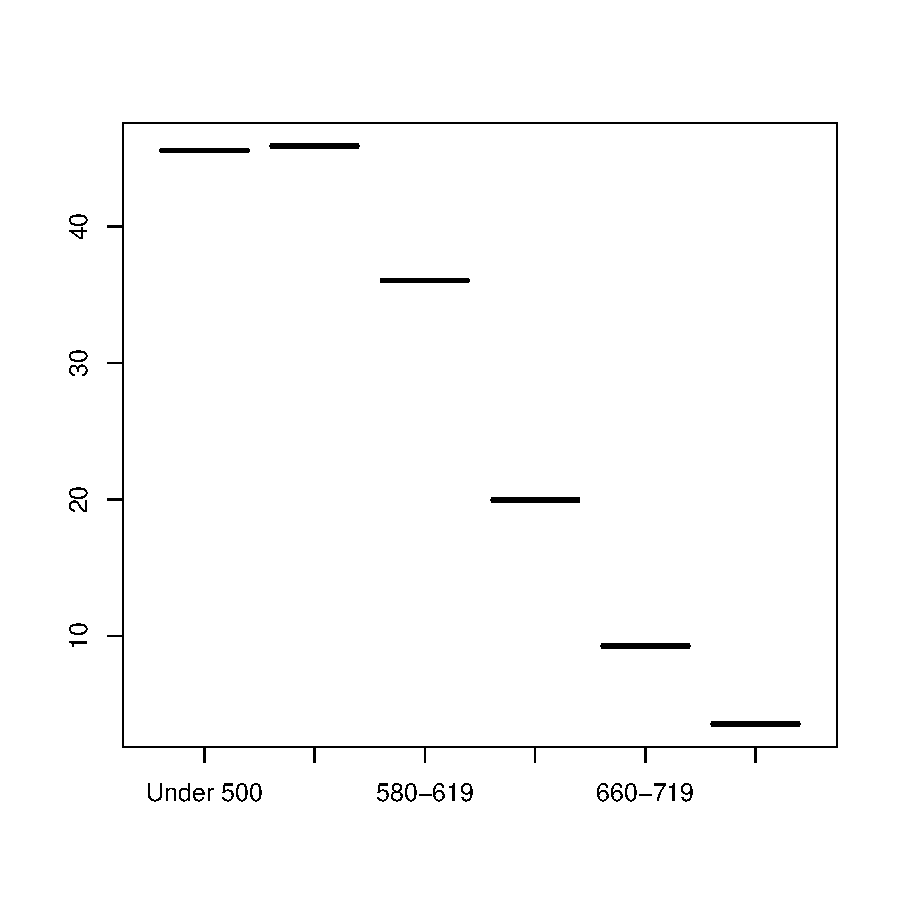
\includegraphics{debseal_HW2-010}
					\end{center}			
			\end{enumerate}				
		\end{enumerate}		
		
	\item[Problem] 5  From Tan, exercises Chapter 2: 2,3,6,12,13,16,19,24.
		\begin{enumerate}
			\item Ex 2 \\
			\emph{Answer:}
			\begin{enumerate}[(a)]
				\item Time in terms of AM and PM. - Binary, qualitative, ordinal
				\item Brightness as measured by a light meter. - Continuous, quantitative,ratio
				\item Brightness as measured by peoples judgments. - Discrete, qualitative,ordinal
				\item Angles as measured in degrees between $0\,^{\circ}$ and $360\,^{\circ}$. - Continuous, quantitative,ratio
				\item Bronze, Silver, and Gold medals as awarded at the Olympics. - Discrete,qualitative, ordinal
				\item Height above sea level. - Continuous, quantitative, interval/ratio*
				\item Number of patients in a hospital. - Discrete, quantitative, ratio
				\item ISBN numbers for books. - Discrete,qualitative, nominal
				\item Ability to pass light in terms of the following values: opaque, translucent,transparent.-Discrete, qualitative, ordinal
				\item Military rank. - Discrete, qualitative, ordinal
				\item Distance from the center of campus. - Continuous, quantitative, interval/ratio*
				\item Density of a substance in grams per cubic centimeter. - Continuous, quantitative,ratio
				\item Coat check number. - Discrete, qualitative, nominal \\
				* It can be observed as interval/ratio based on how you look at them.
			\end{enumerate}

			\item Ex 3 \\
			\emph{Answer:} 
			\begin{enumerate}
				\item Who is right, the marketing director or his boss? If you answered, his boss, what would you do to fix the measure of satisfaction?
				\emph{Answer:} Clearly boss is right here. And apparently the marketing director missed a very obvious thing i.e. The total number of
				people using the product.Since, the product which is being used by many people will have a lot of complaints as well. So a better measure of
				satisfaction would be: \\
				$Measure of Satisfaction = \frac{\text{Number of complaints for the product (say X)}}{\text{Total Number of people using that product X}}$
				
				\item What can you say about the attribute type of the original product satisfaction attribute?\\
				\emph{Answer:} About the original product satisfaction attribute type is little bit confusing. And I cannot come up with any conclusion.
			\end{enumerate}
			\pagebreak
			\item Ex 6 \\
			\emph{Answer:}
				\begin{enumerate}[(a)]
					\item
					Answer: We can have it like below. Having data in binary formation is very important for association analysis.
					\begin{table}[h]
					\caption{Table format for the data} 
					\centering
					\begin{tabular}{l cccc}
						\hline
						Questions & OptionA & OptionB & OptionC & OptionD \\
						\hline
						Question 1 & 0 & 1 & 0 & 0 \\
						Question 2 & 1 & 0 & 0 & 0 \\
						. & . & . & . & .\\
						. & . & . & . & .\\
						. & . & . & . & .\\
						Question 100 & 1 & 0 & 0 & 0 \\
						\hline
					\end{tabular}	
				\end{table}	
				
					\item 
					Answer: Clearly, the attribute type is Binary and they 400 of them.
				\end{enumerate}

			\item Ex 12\\
			\emph{Answer:}
			\begin{enumerate}[(a)]
				\item 
				Answer: Noise is never desirable. On the other hand, Outlier's could be.
				
				\item 
				Answer: Yes definitely. It is resulted due to the distortion of data.
				
				\item 
				Answer: Not necessary. What never know what distortion might do to data.
				
				\item 
				Answer: No. They are part of original data but just not in line with others.
				
				\item 
				Answer: Yes. As i said earlier, we never know what distortion might do to data.
			\end{enumerate}

			\item Ex 13\\
			\emph{Answer:}
			\begin{enumerate}[(a)]
				\item 
				Answer: Firstly, since the distance between the duplicate objects are 0. We would always pick that one among the k nearest 
				neighbour. Also, if duplicates are more. the list may contain of only duplicates. Which does not tell us anything.
				
				\item 
				Answer: One simple but not so good idea is to get rid of them. Or another thing can be, we return not only the distance but also
				some kind of flag, which tells whether the 2 points compared are same or not. 
			\end{enumerate}
			
			\item Ex 16\\
			\emph{Answer:}
			\begin{enumerate}[(a)]
				\item 
				Answer: Clearly, if a word appears just once then, it is of huge importance and same is reflected in the formula and then \\
				$tf^{\prime}_{ij} = tf_{ij} * log m$ \\
				However, when the word appears in all document. Hence, it is of least significance.\\
				$tf^{\prime}_{ij} = tf_{ij} * log 1 \implies 0$\\
				
				\item 
				Answer: As we know IDR is used to classify documents based on words. And a word which appears inevery document like a, the etc. 
				are of no use to us. And this transformation helps us to achieve the same.
			\end{enumerate}
			
			\item Ex 19\\
			\emph{Answer:}
			\begin{table}[h]
					\caption{Calculate the Indicated Similarity} 
					\centering
					\begin{tabular}{l cccc}
						\hline
						Vectors& Cosine & Correlation & Euclidean& Jaccard\\
						\hline
						x = (1, 1, 1, 1), y = (2, 2, 2, 2) & 1 & undefined & 2 & NA\\
						x = $(0,{-}1, 0, 1)$, y = $(1, 0,{-}1, 0)$ & 0 & 0 & 2 & NA\\
						x = (1, 1, 0, 1, 0, 1), y = (1, 1, 1, 0, 0, 1) & 0.75 & 0.25 & 0.6 & NA\\
						x = $(2,{-}1, 0, 2, 0,{-}3)$, y = $({-}1, 1,{-}1, 0, 0,{-}1)$& 0 & 0 & NA & NA\\

						\hline
					\end{tabular}	
				\end{table}	

			\item Ex 24\\
			\emph{Answer:}
			\begin{enumerate}[(a)]
				\item 
				Answer: One possible way could be like K means clustering i.e. find a centroid and compute the distance from that point.Another way
				is to implement pairwise proximity (iteratively).
				
				\item 
				Answer: Once simple way, is to compute the distance between the centroids of the sets.
				
				\item 
				Answer: Once simple way, is to compute the distance between the centroids of the sets.
			\end{enumerate}

		\end{enumerate}
		
\end{enumerate}
\end{document}
